% Created 2016-03-09 Wed 11:21
% Intended LaTeX compiler: pdflatex
\documentclass[11pt]{article}
\usepackage[utf8]{inputenc}
\usepackage[T1]{fontenc}
\usepackage{graphicx}
\usepackage{grffile}
\usepackage{longtable}
\usepackage{wrapfig}
\usepackage{rotating}
\usepackage[normalem]{ulem}
\usepackage{amsmath}
\usepackage{textcomp}
\usepackage{amssymb}
\usepackage{capt-of}
\usepackage{hyperref}
\input article_setup
\usepackage[section]{placeins}
\usepackage{siunitx}
\hypersetup{colorlinks=true,citecolor=cyan,linkcolor=blue,urlcolor=blue}
\author{L. Larrabee Strow}
\date{\today}
\title{AIRS Frequency Calibration Model for L1c}
\hypersetup{
 pdfauthor={L. Larrabee Strow},
 pdftitle={AIRS Frequency Calibration Model for L1c},
 pdfkeywords={},
 pdfsubject={},
 pdfcreator={Emacs 24.5.1 (Org mode 8.3.2)}, 
 pdflang={English}}
\begin{document}

\maketitle

\section{Introduction}
\label{sec:orgheadline1}

This packages contains codes to compute the AIRS channel frequencies
over time.  See \texttt{test\_freqcal.m} for an example of how to use these
codes.  The \texttt{ab.mat} file contains the channel AB states versus time,
there is an entry for every channel property file.  I can provide
the code to read these files if desired.

This package is located on my JPL account in
\texttt{/home/strow/Work/JPL\_nucal}.  You can also get updates from github at
\url(\url{https://github.com/strow/JPL_nucal}).  

\section{Example Run}
\label{sec:orgheadline2}

Run \texttt{test\_freqcal.m} to test.  It will create two plots.  One shows
the change in wavenumber of the center of channel 600 versus time.
The second plot shows the variation in AB state of that channel versus
time.  This channel was chosen since it's AB state changed three
times. 

\section{Status of AIRS Frequency Calibration}
\label{sec:orgheadline3}

I recently measured the AIRS frequency calibration for the M3 module
over time using daily averaged clear-scenes in a narrow latitude band
at the equator, descending node, ocean only.  

The result is shown in the following figure.  This figure basically
confirms that the exponential decay determine from the first 10 years
of orbit is still good enough to use for later times.  

This is preliminary, since I have modified the mean level of the M3
measured frequency calibration to match the output of \texttt{get\_yoff.m}.  I
am working to understand why I had to do this, but I suspect it is
just a programming issue.

\begin{figure}[htb]
\centering
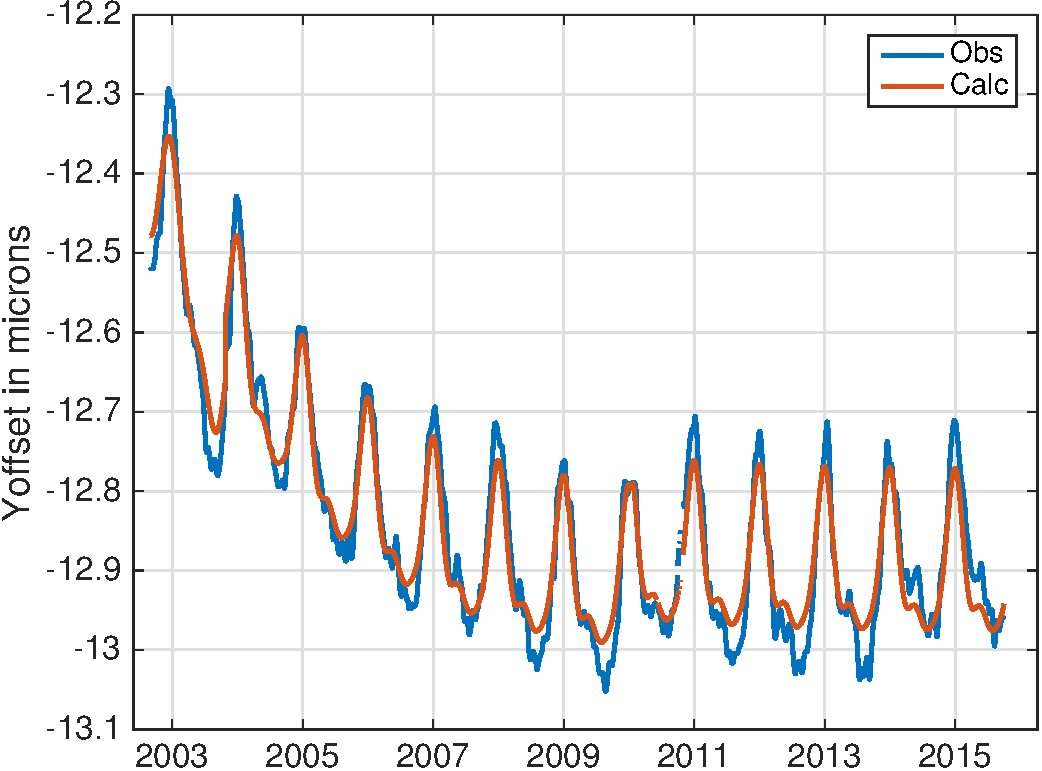
\includegraphics[width=.9\linewidth]{./m3_compare_with_calc_to2015.pdf}
\caption{\label{fig:orgparagraph1}
Relative variation in module M3 from clear-ocean spectra compared to output of get\_yoff.m}
\end{figure}
\end{document}